\documentclass[a4paper, oneside]{memoir}
\usepackage[utf8]{inputenc}
\usepackage[T1]{fontenc}
\usepackage{pifont}
\usepackage{amssymb}
\usepackage{fourier}
\usepackage[dvipsnames]{xcolor}
\usepackage{tikz}
\usepackage{pdfpages}
\usepackage[sfdefault]{roboto}
\usepackage{color}

\tikzstyle{teamshare} = [below, text width=5.4cm, inner sep = 0.5cm, text=white, align=center]
\tikzstyle{cardtext} = [below, text width=5.9cm, inner sep = 0.25cm, text centered]

% Define Commands
\newcommand{\condition}[1]{\textbf{#1}}
\newcommand{\character}[1]{\textbf{#1}}
\newdimen\titlespacing
\titlespacing=0.25cm

% Define Seperators
\newcommand{\redseperator}{\vspace{\titlespacing} \hrulefill {} \ding{100} \hrulefill\\ \vspace{\titlespacing}}
\newcommand{\greenseperator}{\vspace{\titlespacing} \hrulefill {} \bomb{}/\ding{72} \hrulefill\\ \vspace{\titlespacing}}
\newcommand{\greyseperator}{\vspace{\titlespacing} \hrulefill {} \ding{100} \hrulefill\\ \vspace{\titlespacing}}
\newcommand{\purpleseperator}{\vspace{\titlespacing} \hrulefill {} \bomb{}/\ding{72} \hrulefill\\ \vspace{\titlespacing}}
\newcommand{\actionseperator}{\vspace{\titlespacing} \hrulefill {} \tiny power \normalsize \hrulefill\\ \vspace{\titlespacing}}
\newcommand{\descriptionseperator}{\vspace{\titlespacing} \hrulefill {} \tiny description \normalsize \hrulefill\\ \vspace{\titlespacing}}
\newcommand{\modifierseperator}{\vspace{\titlespacing} \hrulefill {} \tiny power \normalsize \hrulefill\\ \vspace{\titlespacing}}
\newcommand{\conditionseperator}{\vspace{\titlespacing} \hrulefill {} \tiny condition \normalsize \hrulefill\\ \vspace{\titlespacing}}
\newcommand{\winseperator}{\vspace{\titlespacing} \hrulefill {} \tiny how to win \normalsize \hrulefill\\ \vspace{\titlespacing}}
\newcommand{\redwinsection}{
	\winseperator
	You win if \character{Santa} does not gain the \condition{humbug} condition due to the \character{Grinch} stealing Christmas.
}
\newcommand{\greenwinsection}{
	\winseperator
	\small You win if \character{Santa} gains the \condition{humbug} condition due to the \character{Grinch} stealing Christmas.
}



%Margin-indstillinger:
\setlrmarginsandblock{0.9cm}{*}{1} %angiver venstre-, så højremargin
\setulmarginsandblock{1.49cm}{*}{1} %angiver øvre-, så nedremargin
\checkandfixthelayout[nearest]

%Følgende giver en minimal sidehoved og sidefod hvor der kun er sidetal.
\pagestyle{empty}

\begin{document}
\noindent 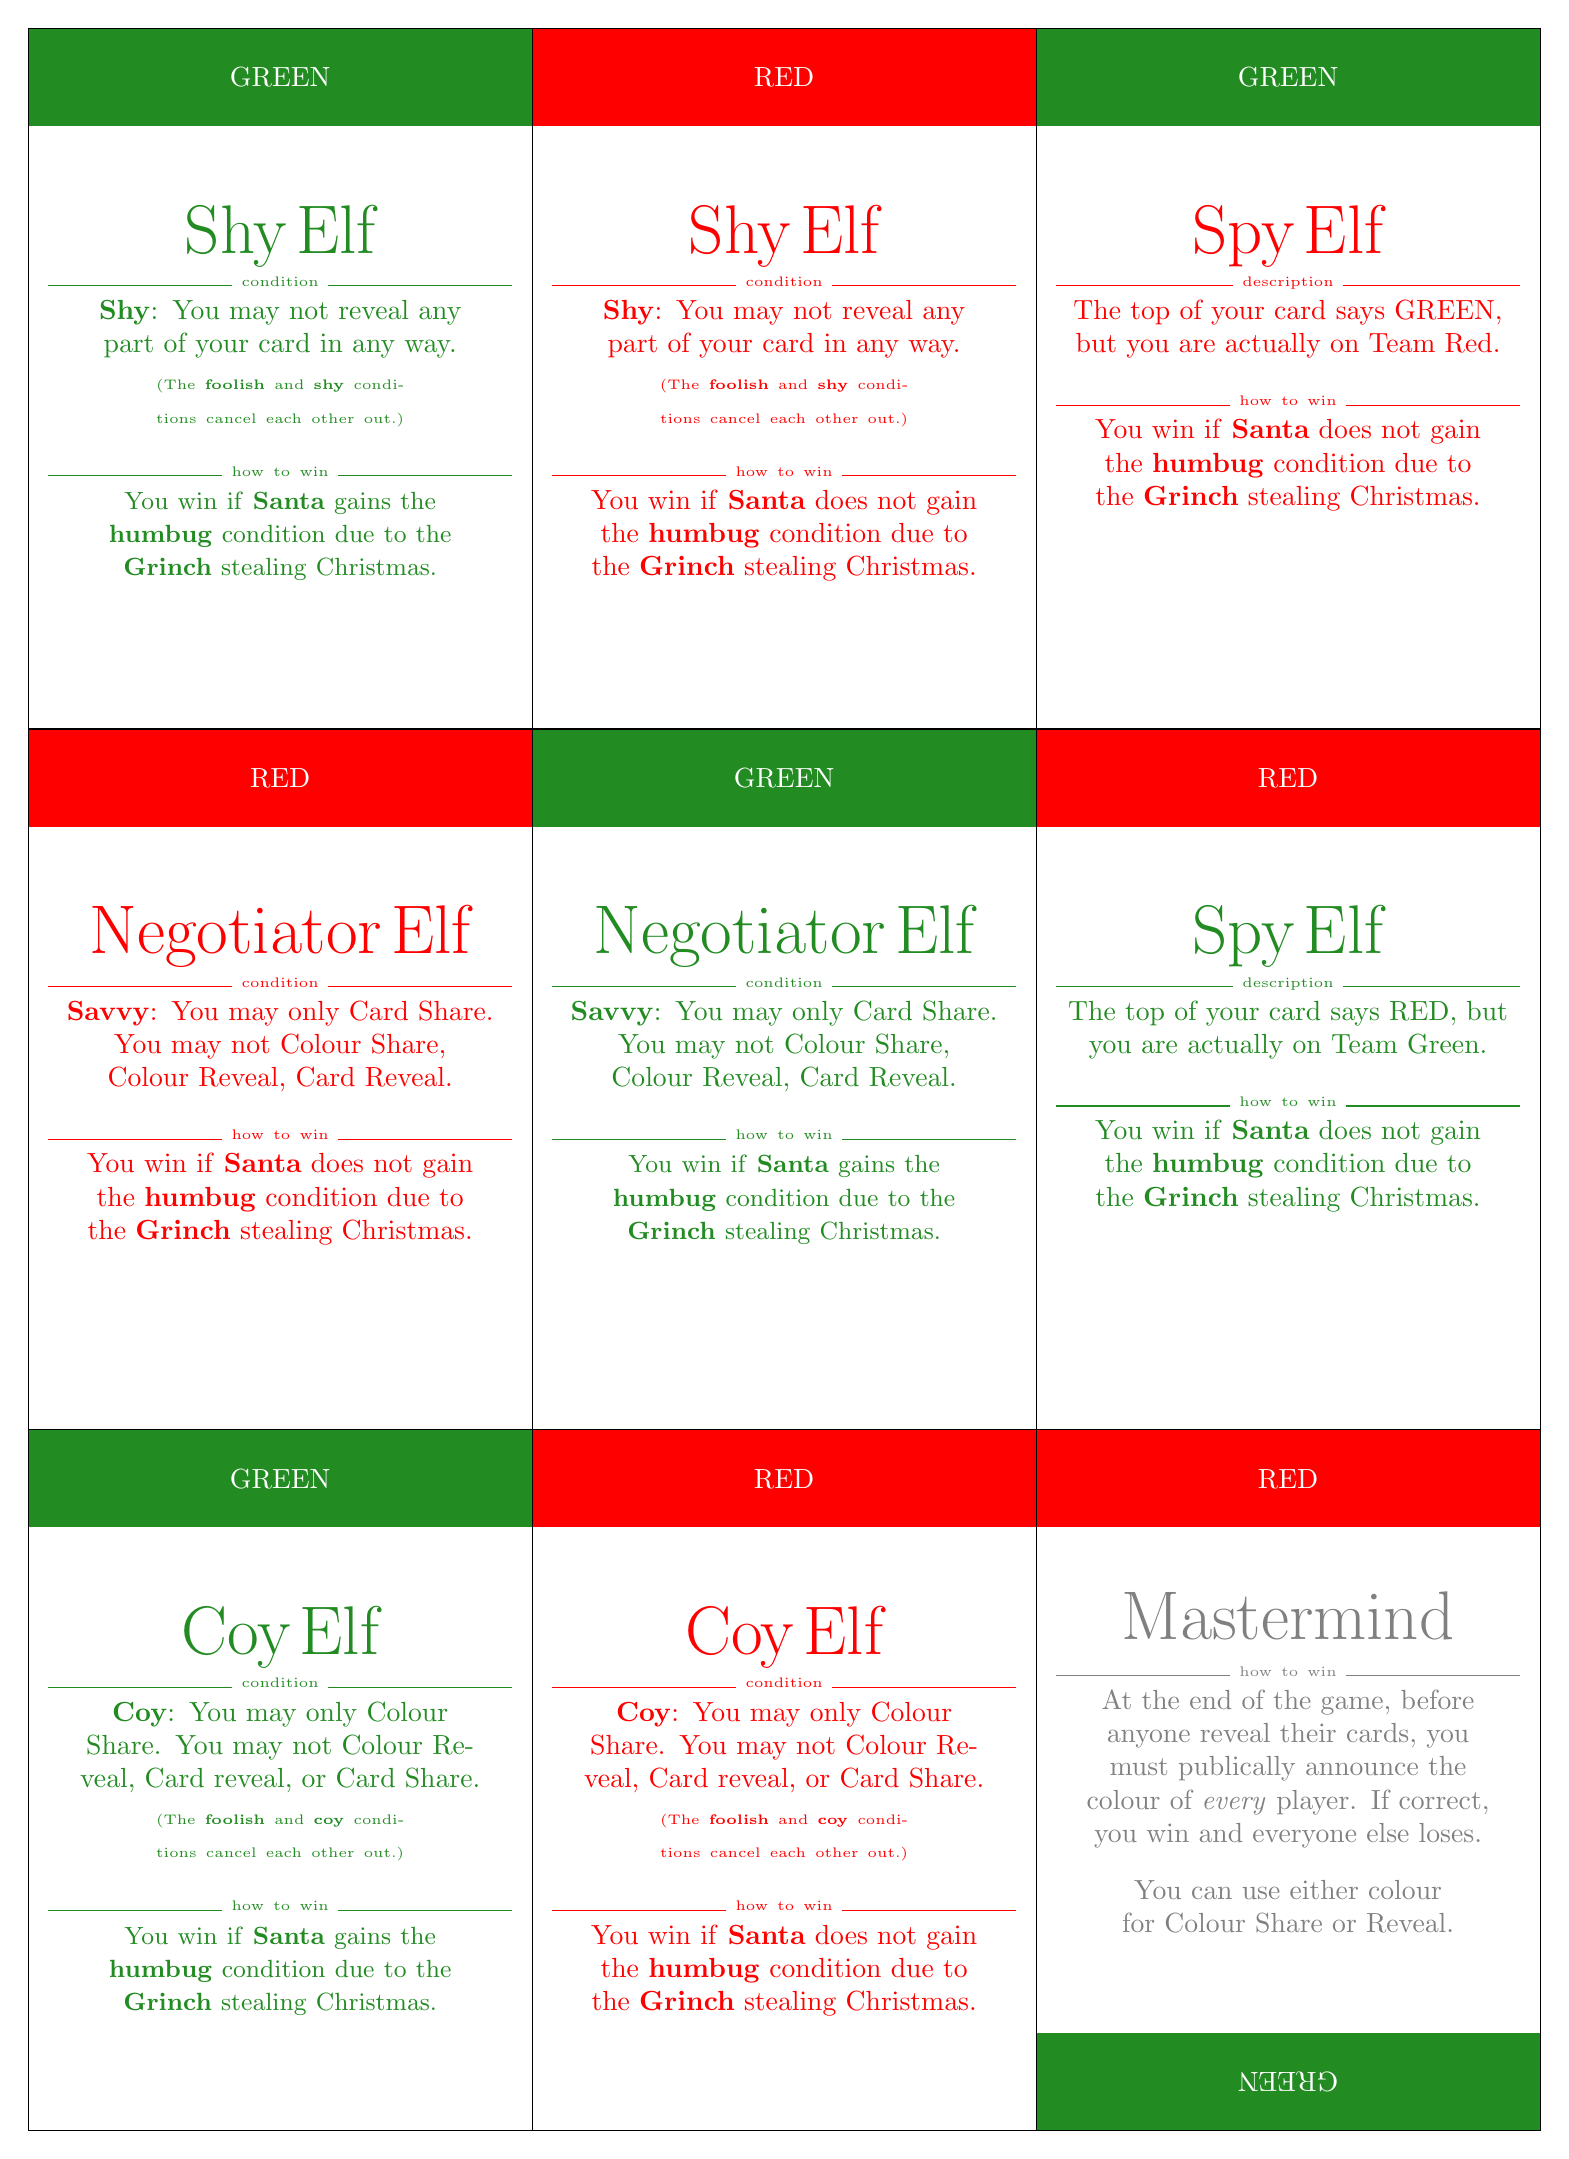
\begin{tikzpicture}[outer sep=0]

% SHY ELF (GREEN TEAM)
\node[teamshare, fill=ForestGreen] (1) at (3.2,26.7) {\HUGE GREEN};
\node[cardtext, text=ForestGreen] at (3.2,24.7) {
	{\Huge Shy Elf}
	\\\conditionseperator
	\condition{Shy}: You may not reveal any part of your card in any way.
	\\\vspace{0.05cm}
	\tiny (The \condition{foolish} and \condition{shy} conditions cancel each other out.) \normalsize
	\\\vspace{0.25cm}
	\greenwinsection
};

% SHY ELF (RED TEAM)
\node[teamshare, fill=red] at (9.6,26.7) {\HUGE RED};
\node[cardtext, text=red] at (9.6,24.7) {
	{\Huge Shy Elf}
	\\\conditionseperator
	\condition{Shy}: You may not reveal any part of your card in any way.
	\\\vspace{0.05cm}
	\tiny (The \condition{foolish} and \condition{shy} conditions cancel each other out.) \normalsize
	\\\vspace{0.25cm}
	\redwinsection
};

% SPY ELF (RED TEAM)
\node[teamshare, fill=ForestGreen] at (16,26.7) {\HUGE GREEN};
\node[cardtext, text=red] at (16,24.7) {
	{\Huge Spy Elf}
	\\\descriptionseperator
	The top of your card says GREEN, but you are actually on Team Red.
	\\\vspace{0.25cm}
	\redwinsection
};

% NEGOTIATOR ELF (RED TEAM)
\node[teamshare, fill=red] at (3.2,17.8) {\HUGE RED};
\node[cardtext, text=red] at (3.2,15.8) {
	{\Huge Negotiator Elf}
	\\\conditionseperator
	\condition{Savvy}: You may only Card Share. You may not Colour Share, Colour Reveal, Card Reveal.
	\\\vspace{0.25cm}
	\redwinsection
};

% NEGOTIATOR ELF (GREEN TEAM)
\node[teamshare, fill=ForestGreen] at (9.6,17.8) {\HUGE GREEN};
\node[cardtext, text=ForestGreen] at (9.6,15.8) {
	{\Huge Negotiator Elf}
	\\\conditionseperator
	\condition{Savvy}: You may only Card Share. You may not Colour Share, Colour Reveal, Card Reveal.
	\\\vspace{0.25cm}
	\greenwinsection
};

% SPY ELF (GREEN TEAM)
\node[teamshare, fill=red] at (16,17.8) {\HUGE RED};
\node[cardtext, text=ForestGreen] at (16,15.8) {
	{\Huge Spy Elf}
	\\\descriptionseperator
	The top of your card says RED, but you are actually on Team Green.
	\\\vspace{0.25cm}
	\redwinsection
};

% COY ELF (GREEN TEAM)
\node[teamshare, fill=ForestGreen] at (3.2,8.9) {\HUGE GREEN};
\node[cardtext, text=ForestGreen] at (3.2,6.9) {
	{\Huge Coy Elf}
	\\\conditionseperator
	\condition{Coy}: You may only Colour Share. You may not Colour Reveal, Card reveal, or Card Share.
	\\\vspace{0.05cm}
	\tiny (The \condition{foolish} and \condition{coy} conditions cancel each other out.) \normalsize
	\\\vspace{0.25cm}
	\greenwinsection
};

% COY ELF (RED TEAM)
\node[teamshare, fill=red] at (9.6,8.9) {\HUGE RED};
\node[cardtext, text=red] at (9.6,6.9) {
	{\Huge Coy Elf}
	\\\conditionseperator
	\condition{Coy}: You may only Colour Share. You may not Colour Reveal, Card reveal, or Card Share.
	\\\vspace{0.05cm}
	\tiny (The \condition{foolish} and \condition{coy} conditions cancel each other out.) \normalsize
	\\\vspace{0.25cm}
	\redwinsection
};

% MASTERMIND
\node[teamshare, fill=red] at (16,8.9) {\HUGE RED};
\node[teamshare, fill=ForestGreen,rotate=180] at (16,0) {\HUGE GREEN};
\node[cardtext, text=gray] at (16,7.1) {
	{\Huge Mastermind}
	\\\vspace{0.05cm}
	\winseperator
	At the end of the game, before anyone reveal their cards, you must publically announce the colour of \emph{every} player. If correct, you win and everyone else loses.
	\\\vspace{0.3cm}
	You can use either colour for Colour Share or Reveal.
};

\draw (0,0) -- (19.2,0);
\draw (0,8.9) -- (19.2,8.9);
\draw (0,17.8) -- (19.2,17.8);
\draw (0,26.7) -- (19.2,26.7);

\draw (0,0) -- (0,26.7);
\draw (6.4,0) -- (6.4,26.7);
\draw (12.8,0) -- (12.8,26.7);
\draw (19.2,0) -- (19.2,26.7);



\end{tikzpicture}

%Background is not my own. But courtesy of a user on BGG

\includepdf[pages={1}, angle=90]{cardsbackground.pdf}
\pagebreak





\noindent 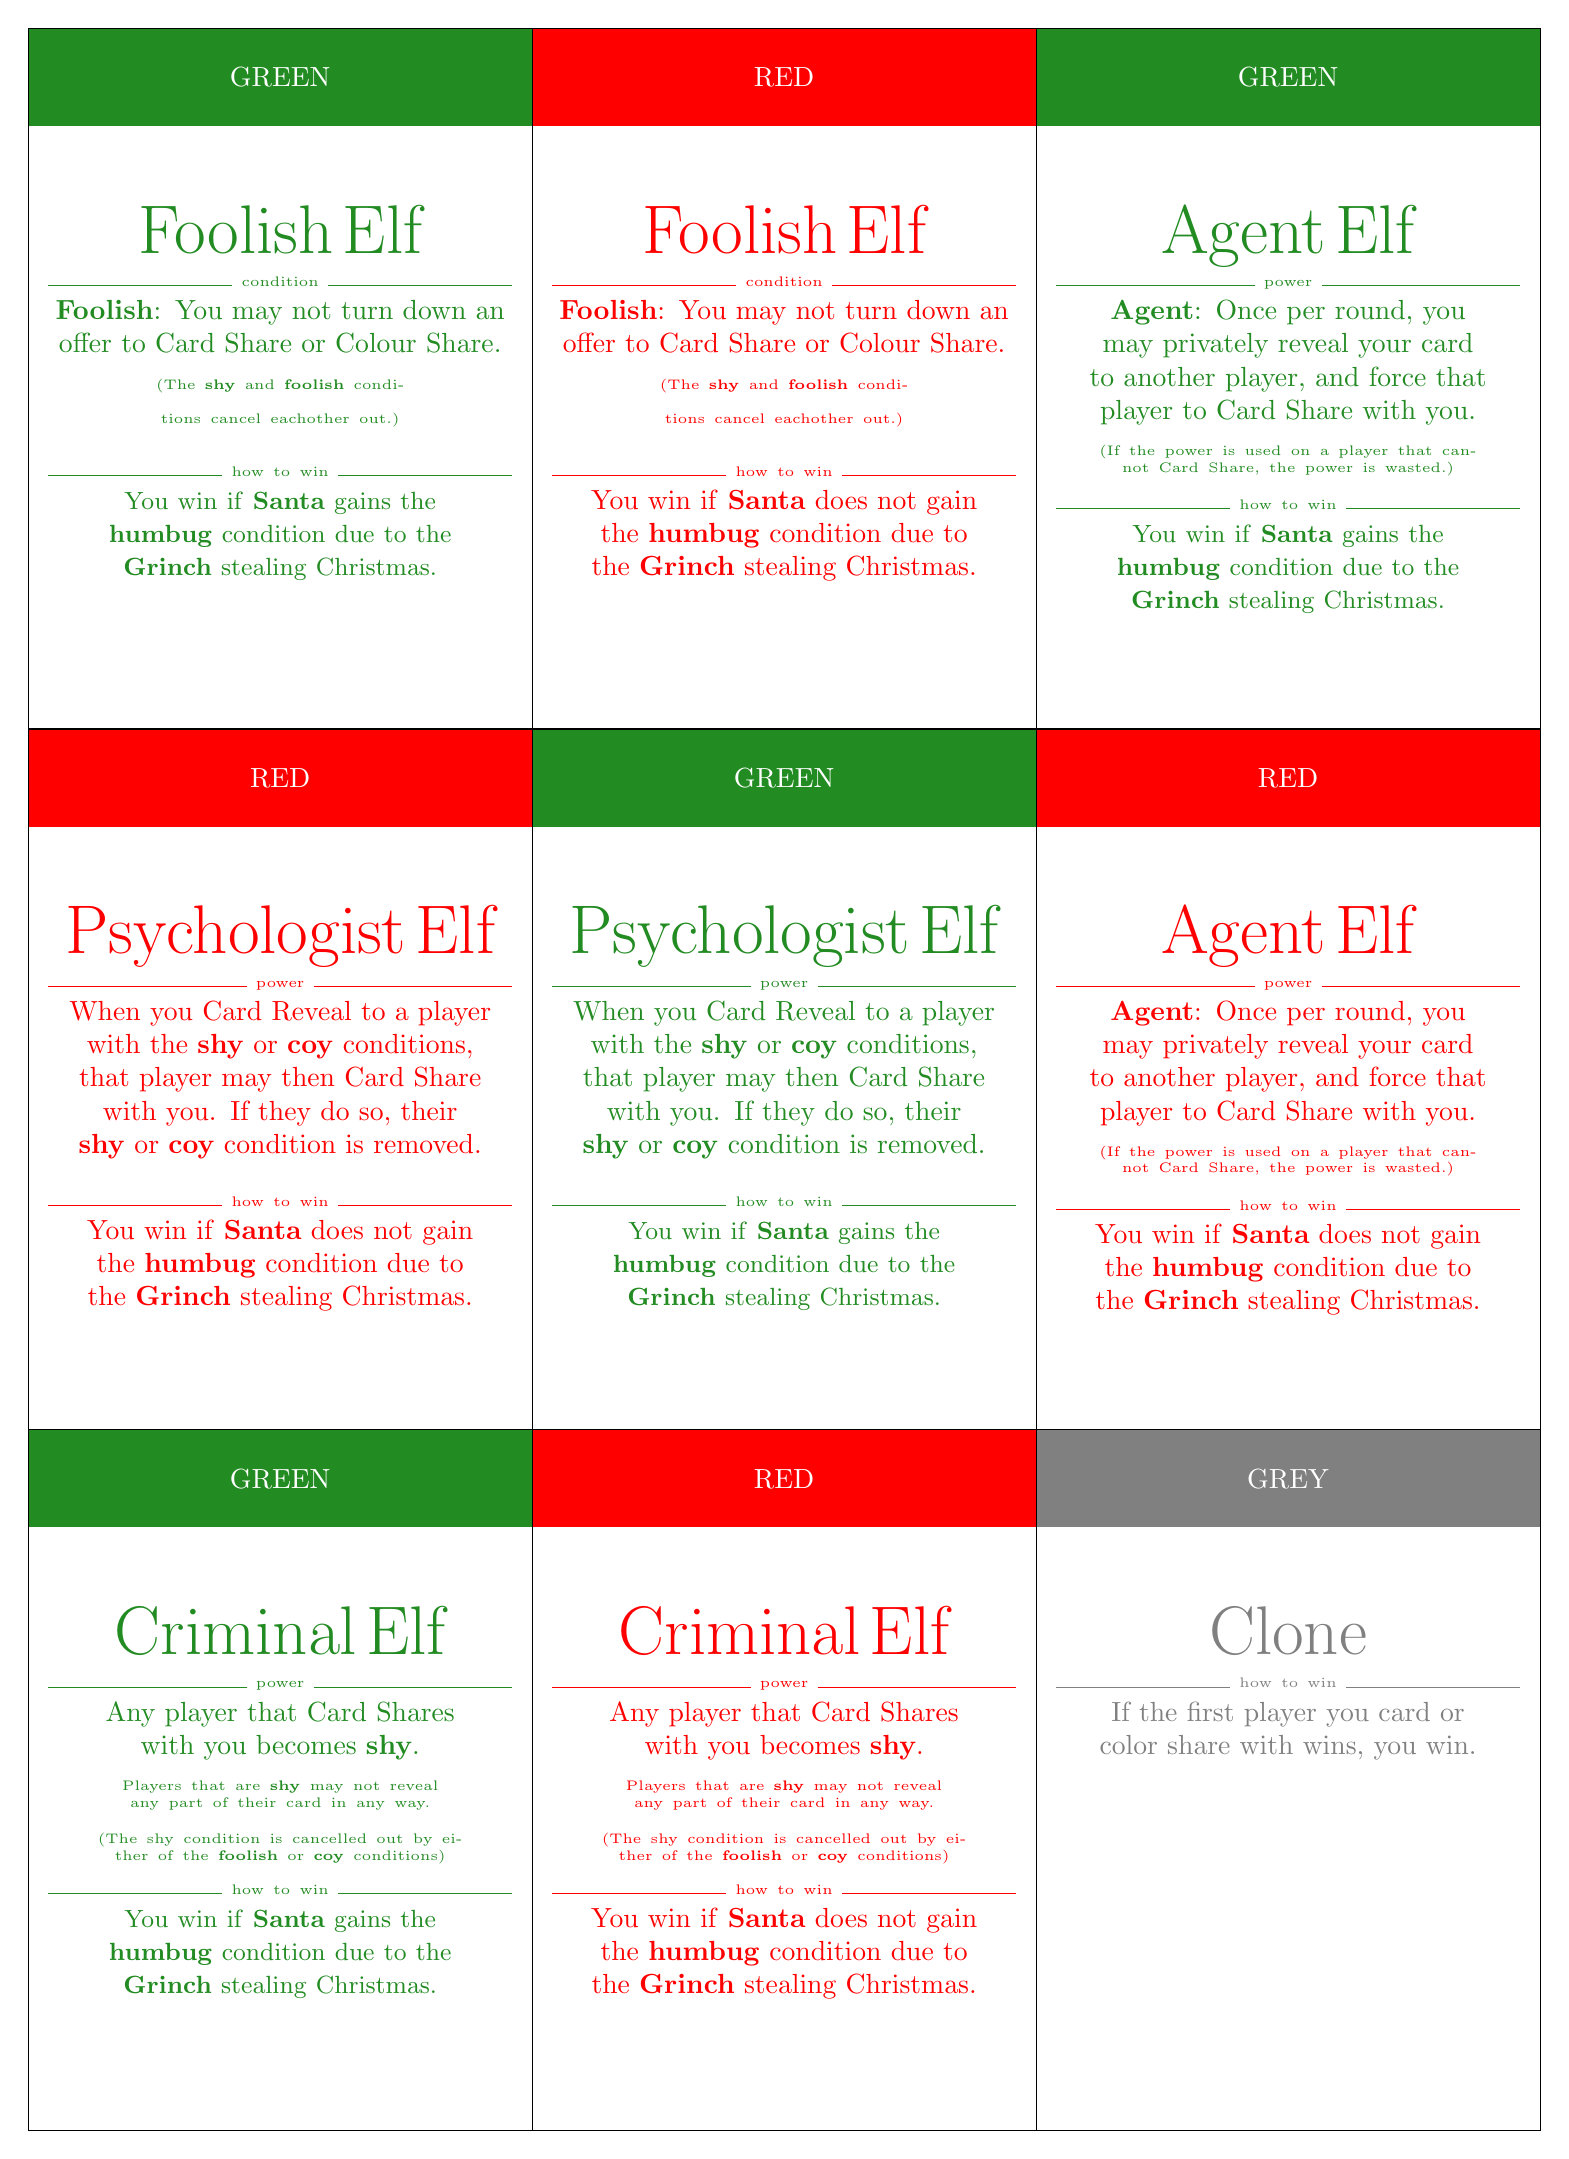
\begin{tikzpicture}[outer sep=0]

% Foolish Elf (Green Team)
\node[teamshare, fill=ForestGreen] (1) at (3.2,26.7) {\HUGE GREEN};
\node[cardtext, text=ForestGreen] at (3.2,24.7) {
	{\Huge Foolish Elf}
	\\\conditionseperator
	\condition{Foolish}: You may not turn down an offer to Card Share or Colour Share.
	\\\vspace{0.05cm}
	\tiny (The \condition{shy} and \condition{foolish} conditions cancel eachother out.) \normalsize
	\\\vspace{0.25cm}
	\greenwinsection
};

% FOOLISH ELF (RED TEAM)
\node[teamshare, fill=red] at (9.6,26.7) {\HUGE RED};
\node[cardtext, text=red] at (9.6,24.7) {
	{\Huge Foolish Elf}
	\\\conditionseperator
	\condition{Foolish}: You may not turn down an offer to Card Share or Colour Share.
	\\\vspace{0.05cm}
	\tiny (The \condition{shy} and \condition{foolish} conditions cancel eachother out.) \normalsize
	\\\vspace{0.25cm}
	\redwinsection
};

% AGENT ELF (GREEN TEAM)
\node[teamshare, fill=ForestGreen] at (16,26.7) {\HUGE GREEN};
\node[cardtext, text=ForestGreen] at (16,24.7) {
	{\Huge Agent Elf}
	\\\actionseperator
	\condition{Agent}: Once per round, you may privately reveal your card to another player, and force that player to Card Share with you.
	\\\vspace{0.25cm}
	\tiny (If the power is used on a player that cannot Card Share, the power is wasted.)
	\\\vspace{0.05cm}
	\greenwinsection
};

% PSYCHOLOGIST ELF (RED TEAM)
\node[teamshare, fill=red] at (3.2,17.8) {\HUGE RED};
\node[cardtext, text=red] at (3.2,15.8) {
	{\Huge Psychologist Elf}
	\\\modifierseperator
	When you Card Reveal to a player with the \condition{shy} or \condition{coy} conditions, that player may then Card Share with you. If they do so, their \condition{shy} or \condition{coy} condition is removed.
	\\\vspace{0.25cm}
	\redwinsection
};

% PSYCHOLOGIST ELF (GREEN TEAM)
\node[teamshare, fill=ForestGreen] at (9.6,17.8) {\HUGE GREEN};
\node[cardtext, text=ForestGreen] at (9.6,15.8) {
	{\Huge Psychologist Elf}
	\\\modifierseperator
	When you Card Reveal to a player with the \condition{shy} or \condition{coy} conditions, that player may then Card Share with you. If they do so, their \condition{shy} or \condition{coy} condition is removed.
	\\\vspace{0.25cm}
	\greenwinsection
};

% AGENT ELF (RED TEAM)
\node[teamshare, fill=red] at (16,17.8) {\HUGE RED};
\node[cardtext, text=red] at (16,15.8) {
	{\Huge Agent Elf}
	\\\actionseperator
	\condition{Agent}: Once per round, you may privately reveal your card to another player, and force that player to Card Share with you.
	\\\vspace{0.25cm}
	\tiny (If the power is used on a player that cannot Card Share, the power is wasted.)
	\\\vspace{0.05cm}
	\redwinsection
};

% CRIMINAL ELF (GREEN TEAM)
\node[teamshare, fill=ForestGreen] at (3.2,8.9) {\HUGE GREEN};
\node[cardtext, text=ForestGreen] at (3.2,6.9) {
	{\Huge Criminal Elf}
	\\\modifierseperator
	Any player that Card Shares with you becomes \condition{shy}.
	\\\vspace{0.25cm}
	\tiny Players that are \condition{shy} may not reveal any part of their card in any way.
	\\\vspace{0.25cm}
	\tiny (The shy condition is cancelled out by either of the \condition{foolish} or \condition{coy} conditions)
	\\\vspace{0.01cm}
	\greenwinsection
};

% CRIMINAL ELF (RED TEAM)
\node[teamshare, fill=red] at (9.6,8.9) {\HUGE RED};
\node[cardtext, text=red] at (9.6,6.9) {
	{\Huge Criminal Elf}
	\\\modifierseperator
	Any player that Card Shares with you becomes \condition{shy}.
	\\\vspace{0.25cm}
	\tiny Players that are \condition{shy} may not reveal any part of their card in any way.
	\\\vspace{0.25cm}
	\tiny (The shy condition is cancelled out by either of the \condition{foolish} or \condition{coy} conditions)
	\\\vspace{0.01cm}
	\redwinsection
};

% CLONE
\node[teamshare, fill=gray] at (16,8.9) {\HUGE GREY};
\node[cardtext, text=gray] at (16,6.9) {
	{\Huge Clone}
	\\\winseperator
	If the first player you card or color share with wins, you win.
};

\draw (0,0) -- (19.2,0);
\draw (0,8.9) -- (19.2,8.9);
\draw (0,17.8) -- (19.2,17.8);
\draw (0,26.7) -- (19.2,26.7);

\draw (0,0) -- (0,26.7);
\draw (6.4,0) -- (6.4,26.7);
\draw (12.8,0) -- (12.8,26.7);
\draw (19.2,0) -- (19.2,26.7);



\end{tikzpicture}

%Background is not my own. But courtesy of a user on BGG

\includepdf[pages={1}, angle=90]{cardsbackground.pdf}







\noindent 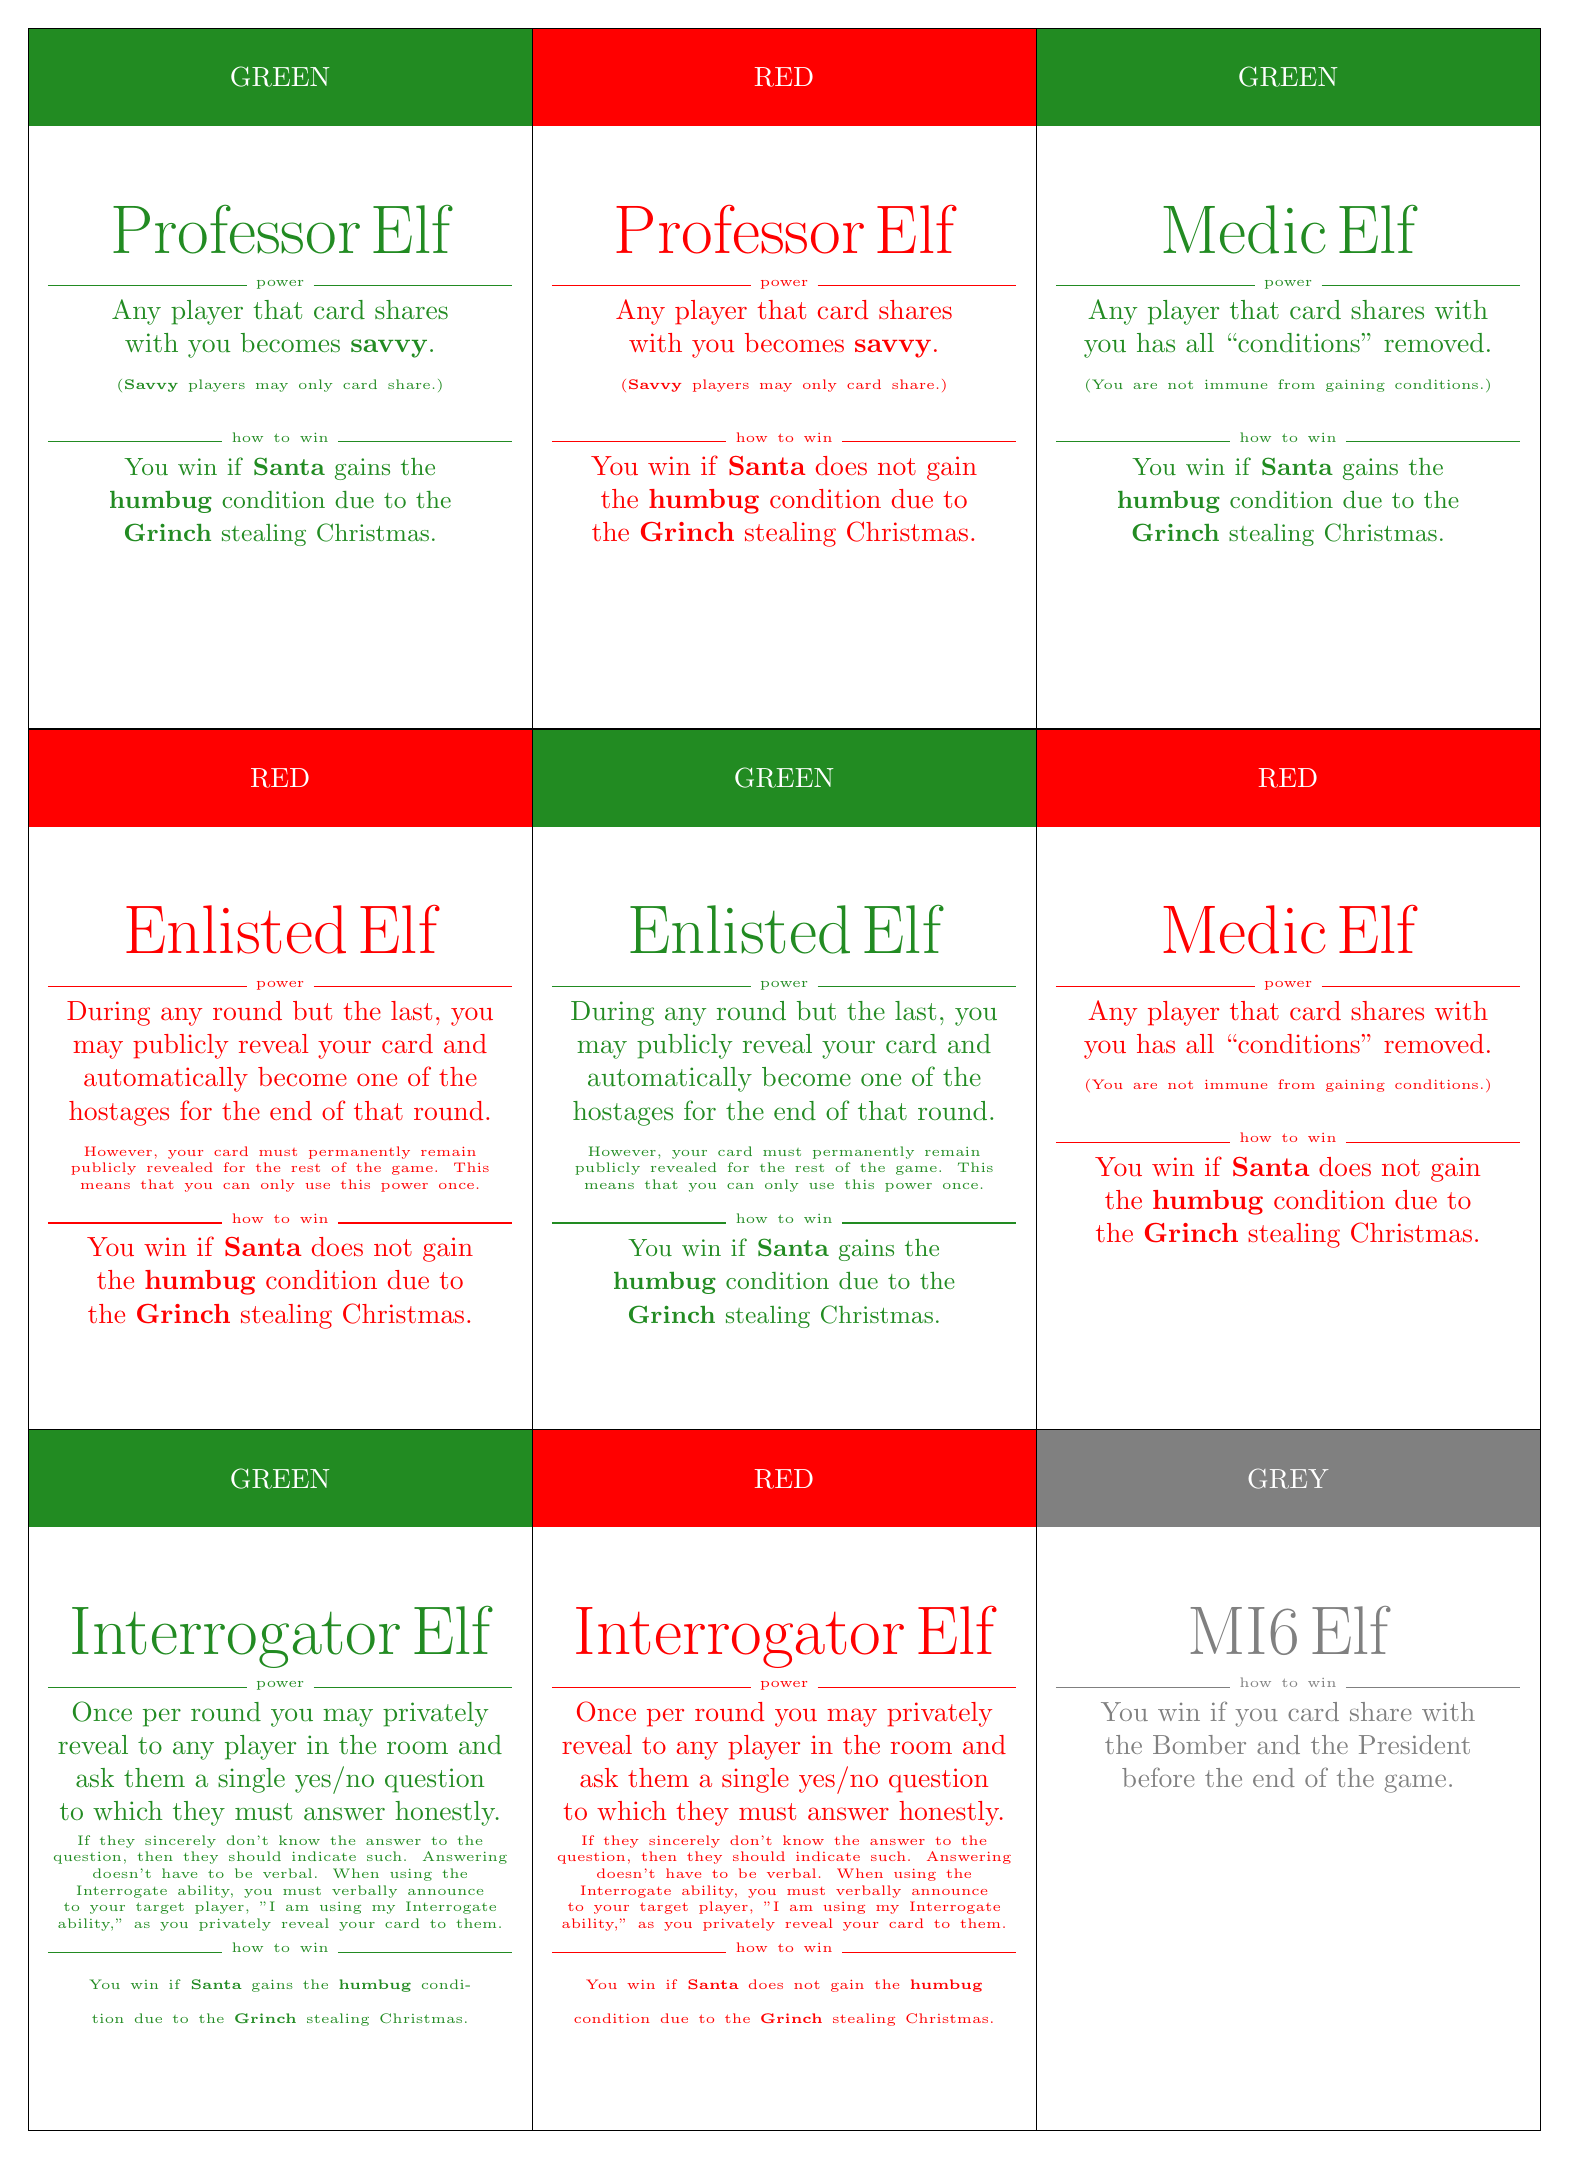
\begin{tikzpicture}[outer sep=0]

% PROFESSOR ELF (GREEN TEAM)
\node[teamshare, fill=ForestGreen] (1) at (3.2,26.7) {\HUGE GREEN};
\node[cardtext, text=ForestGreen] at (3.2,24.7) {
	{\Huge Professor Elf}
	\\\actionseperator
	Any player that card shares with you becomes \condition{savvy}.
	\\\vspace{0.25cm}
	\tiny (\condition{Savvy} players may only card share.)
	\\\vspace{0.25cm}
	\greenwinsection
};

% PROFESSOR ELF (RED TEAM)
\node[teamshare, fill=red] at (9.6,26.7) {\HUGE RED};
\node[cardtext, text=red] at (9.6,24.7) {
	{\Huge Professor Elf}
	\\\actionseperator
	Any player that card shares with you becomes \condition{savvy}.
	\\\vspace{0.25cm}
	\tiny (\condition{Savvy} players may only card share.)
	\\\vspace{0.25cm}
	\redwinsection
};

% MEDIC ELF (RED TEAM)
\node[teamshare, fill=ForestGreen] at (16,26.7) {\HUGE GREEN};
\node[cardtext, text=ForestGreen] at (16,24.7) {
	{\Huge Medic Elf}
	\\\actionseperator
	Any player that card shares with you has all “conditions” removed.
	\\\vspace{0.25cm}
	\tiny (You are not immune from gaining conditions.)
	\\\vspace{0.25cm}
	\greenwinsection
};

% ENLISTED ELF (RED TEAM)
\node[teamshare, fill=red] at (3.2,17.8) {\HUGE RED};
\node[cardtext, text=red] at (3.2,15.8) {
	{\Huge Enlisted Elf}
	\\\actionseperator
	During any round but the last, you may publicly reveal your card and automatically become one of the hostages for the end of that round. 
	\\\vspace{0.25cm}
	\tiny However, your card must permanently remain publicly revealed for the rest of the game. This means that you can only use this power once.
	\\\vspace{0.01cm}
	\redwinsection
};

% ENLISTED ELF (GREEN TEAM)
\node[teamshare, fill=ForestGreen] at (9.6,17.8) {\HUGE GREEN};
\node[cardtext, text=ForestGreen] at (9.6,15.8) {
	{\Huge Enlisted Elf}
	\\\actionseperator
	During any round but the last, you may publicly reveal your card and automatically become one of the hostages for the end of that round. 
	\\\vspace{0.25cm}
	\tiny However, your card must permanently remain publicly revealed for the rest of the game. This means that you can only use this power once.
	\\\vspace{0.01cm}
	\greenwinsection
};

% MEDIC ELF (RED TEAM)
\node[teamshare, fill=red] at (16,17.8) {\HUGE RED};
\node[cardtext, text=red] at (16,15.8) {
	{\Huge Medic Elf}
	\\\actionseperator
	Any player that card shares with you has all “conditions” removed.
	\\\vspace{0.25cm}
	\tiny (You are not immune from gaining conditions.)
	\\\vspace{0.25cm}
	\redwinsection
};

% INTERROGATOR ELF (GREEN TEAM)
\node[teamshare, fill=ForestGreen] at (3.2,8.9) {\HUGE GREEN};
\node[cardtext, text=ForestGreen] at (3.2,6.9) {
	{\Huge Interrogator Elf}
	\\\actionseperator
	Once per round you may privately reveal to any player in the room and ask them a single yes/no question to which they must answer honestly.
	\\\vspace{0.1cm} 
	\tiny
	If they sincerely don’t know the answer to the question, then they should indicate such. Answering doesn’t have to be verbal. When using the Interrogate ability, you must verbally announce to your target player, "I am using my Interrogate ability," as you privately reveal your card to them.
	\\\vspace{0.1cm}
	\hrulefill {} \tiny how to win \hrulefill
	\\\vspace{0.05cm}
	\tiny You win if \character{Santa} gains the \condition{humbug} condition due to the \character{Grinch} stealing Christmas.
};

% INTERROGATOR ELF (RED TEAM)
\node[teamshare, fill=red] at (9.6,8.9) {\HUGE RED};
\node[cardtext, text=red] at (9.6,6.9) {
	{\Huge Interrogator Elf}
	\\\actionseperator
	Once per round you may privately reveal to any player in the room and ask them a single yes/no question to which they must answer honestly.
	\\\vspace{0.1cm} 
	\tiny
	If they sincerely don’t know the answer to the question, then they should indicate such. Answering doesn’t have to be verbal. When using the Interrogate ability, you must verbally announce to your target player, "I am using my Interrogate ability," as you privately reveal your card to them.
	\\\vspace{0.1cm}
	\hrulefill {} \tiny how to win \hrulefill
	\\\vspace{0.05cm}
	\tiny You win if \character{Santa} does not gain the \condition{humbug} condition due to the \character{Grinch} stealing Christmas.
};

% MI6 ELF
\node[teamshare, fill=gray] at (16,8.9) {\HUGE GREY};
\node[cardtext, text=gray] at (16,6.9) {
	{\Huge MI6 Elf}
	\\\winseperator
	You win if you card share with the Bomber and the President before the end of the game.
};

\draw (0,0) -- (19.2,0);
\draw (0,8.9) -- (19.2,8.9);
\draw (0,17.8) -- (19.2,17.8);
\draw (0,26.7) -- (19.2,26.7);

\draw (0,0) -- (0,26.7);
\draw (6.4,0) -- (6.4,26.7);
\draw (12.8,0) -- (12.8,26.7);
\draw (19.2,0) -- (19.2,26.7);



\end{tikzpicture}

%Background is not my own. But courtesy of a user on BGG

\includepdf[pages={1}, angle=90]{cardsbackground.pdf}
\pagebreak

\noindent 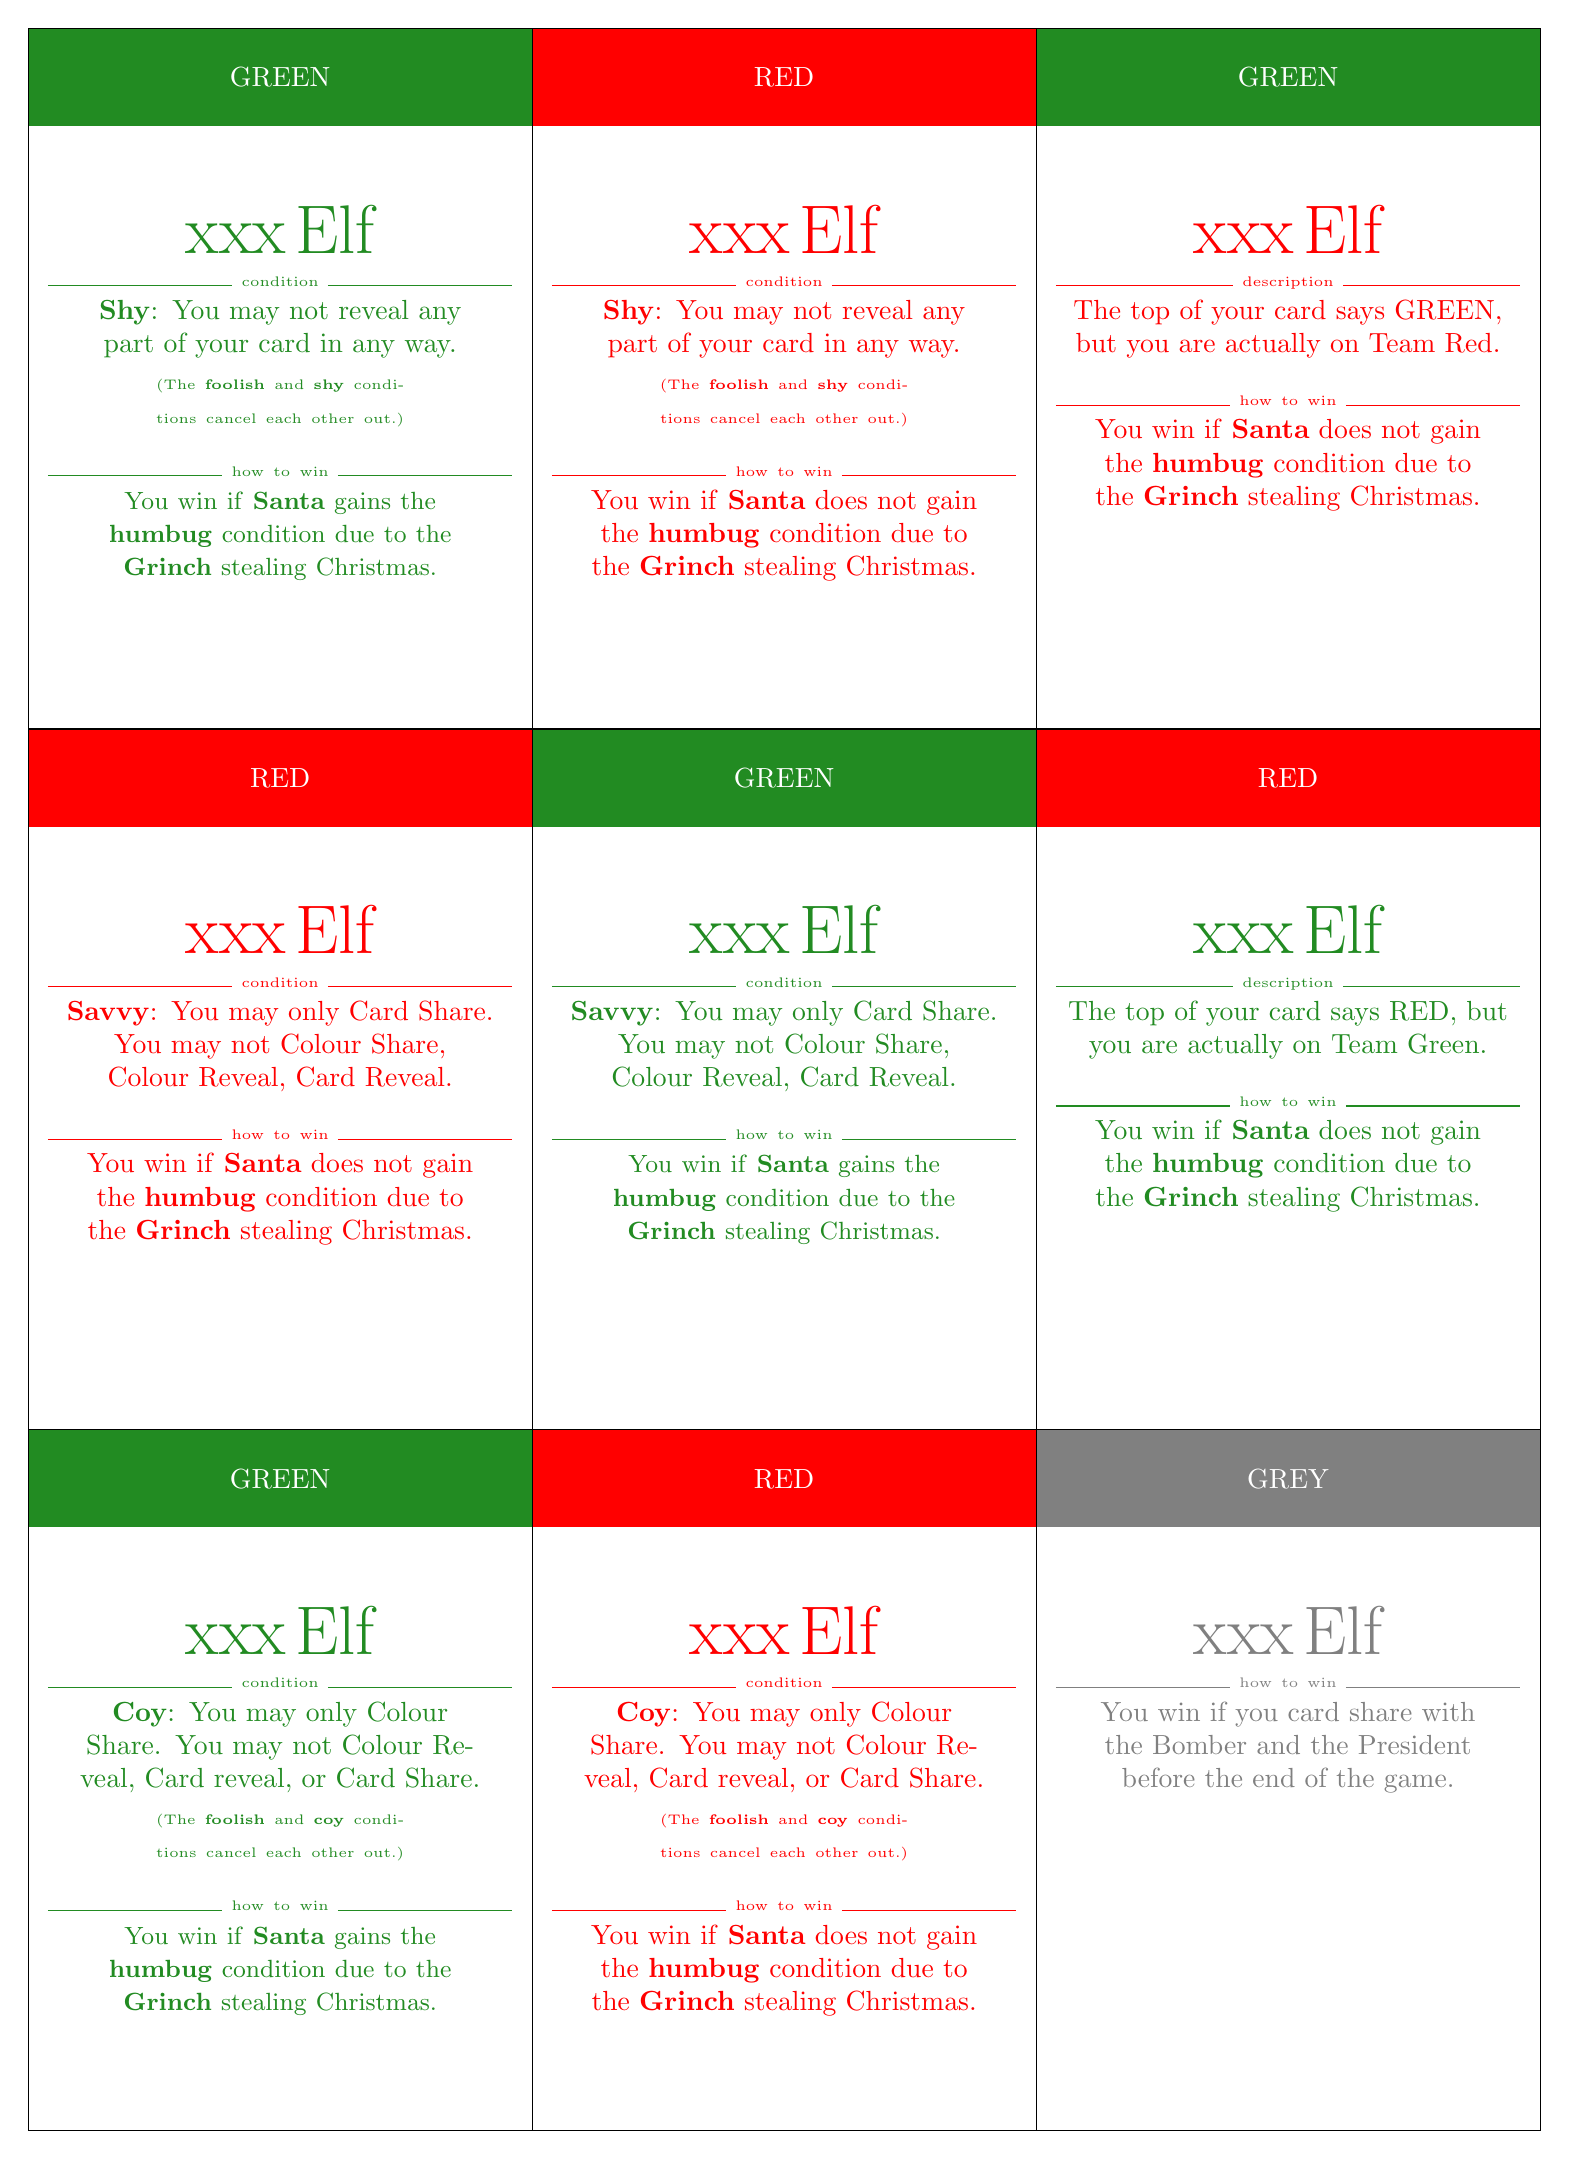
\begin{tikzpicture}[outer sep=0]

% xxx ELF (GREEN TEAM)
\node[teamshare, fill=ForestGreen] (1) at (3.2,26.7) {\HUGE GREEN};
\node[cardtext, text=ForestGreen] at (3.2,24.7) {
	{\Huge xxx Elf}
	\\\conditionseperator
	\condition{Shy}: You may not reveal any part of your card in any way.
	\\\vspace{0.05cm}
	\tiny (The \condition{foolish} and \condition{shy} conditions cancel each other out.) \normalsize
	\\\vspace{0.25cm}
	\greenwinsection
};

% xxx ELF (RED TEAM)
\node[teamshare, fill=red] at (9.6,26.7) {\HUGE RED};
\node[cardtext, text=red] at (9.6,24.7) {
	{\Huge xxx Elf}
	\\\conditionseperator
	\condition{Shy}: You may not reveal any part of your card in any way.
	\\\vspace{0.05cm}
	\tiny (The \condition{foolish} and \condition{shy} conditions cancel each other out.) \normalsize
	\\\vspace{0.25cm}
	\redwinsection
};

% xxx ELF (RED TEAM)
\node[teamshare, fill=ForestGreen] at (16,26.7) {\HUGE GREEN};
\node[cardtext, text=red] at (16,24.7) {
	{\Huge xxx Elf}
	\\\descriptionseperator
	The top of your card says GREEN, but you are actually on Team Red.
	\\\vspace{0.25cm}
	\redwinsection
};

% xxx ELF (RED TEAM)
\node[teamshare, fill=red] at (3.2,17.8) {\HUGE RED};
\node[cardtext, text=red] at (3.2,15.8) {
	{\Huge xxx Elf}
	\\\conditionseperator
	\condition{Savvy}: You may only Card Share. You may not Colour Share, Colour Reveal, Card Reveal.
	\\\vspace{0.25cm}
	\redwinsection
};

% xxx ELF (GREEN TEAM)
\node[teamshare, fill=ForestGreen] at (9.6,17.8) {\HUGE GREEN};
\node[cardtext, text=ForestGreen] at (9.6,15.8) {
	{\Huge xxx Elf}
	\\\conditionseperator
	\condition{Savvy}: You may only Card Share. You may not Colour Share, Colour Reveal, Card Reveal.
	\\\vspace{0.25cm}
	\greenwinsection
};

% xxx ELF (GREEN TEAM)
\node[teamshare, fill=red] at (16,17.8) {\HUGE RED};
\node[cardtext, text=ForestGreen] at (16,15.8) {
	{\Huge xxx Elf}
	\\\descriptionseperator
	The top of your card says RED, but you are actually on Team Green.
	\\\vspace{0.25cm}
	\redwinsection
};

% xxx ELF (GREEN TEAM)
\node[teamshare, fill=ForestGreen] at (3.2,8.9) {\HUGE GREEN};
\node[cardtext, text=ForestGreen] at (3.2,6.9) {
	{\Huge xxx Elf}
	\\\conditionseperator
	\condition{Coy}: You may only Colour Share. You may not Colour Reveal, Card reveal, or Card Share.
	\\\vspace{0.05cm}
	\tiny (The \condition{foolish} and \condition{coy} conditions cancel each other out.) \normalsize
	\\\vspace{0.25cm}
	\greenwinsection
};

% xxx ELF (RED TEAM)
\node[teamshare, fill=red] at (9.6,8.9) {\HUGE RED};
\node[cardtext, text=red] at (9.6,6.9) {
	{\Huge xxx Elf}
	\\\conditionseperator
	\condition{Coy}: You may only Colour Share. You may not Colour Reveal, Card reveal, or Card Share.
	\\\vspace{0.05cm}
	\tiny (The \condition{foolish} and \condition{coy} conditions cancel each other out.) \normalsize
	\\\vspace{0.25cm}
	\redwinsection
};

% xxx ELF
\node[teamshare, fill=gray] at (16,8.9) {\HUGE GREY};
\node[cardtext, text=gray] at (16,6.9) {
	{\Huge xxx Elf}
	\\\winseperator
	You win if you card share with the Bomber and the President before the end of the game.
};


\draw (0,0) -- (19.2,0);
\draw (0,8.9) -- (19.2,8.9);
\draw (0,17.8) -- (19.2,17.8);
\draw (0,26.7) -- (19.2,26.7);

\draw (0,0) -- (0,26.7);
\draw (6.4,0) -- (6.4,26.7);
\draw (12.8,0) -- (12.8,26.7);
\draw (19.2,0) -- (19.2,26.7);



\end{tikzpicture}

%Background is not my own. But courtesy of a user on BGG

\includepdf[pages={1}, angle=90]{cardsbackground.pdf}
\pagebreak





\end{document}